\documentclass[../document.tex]{subfiles}
\begin{document}\label{ssec:energy}

\begin{figure*}
\begin{subfigure}[htb]{.45\textwidth}
\centering
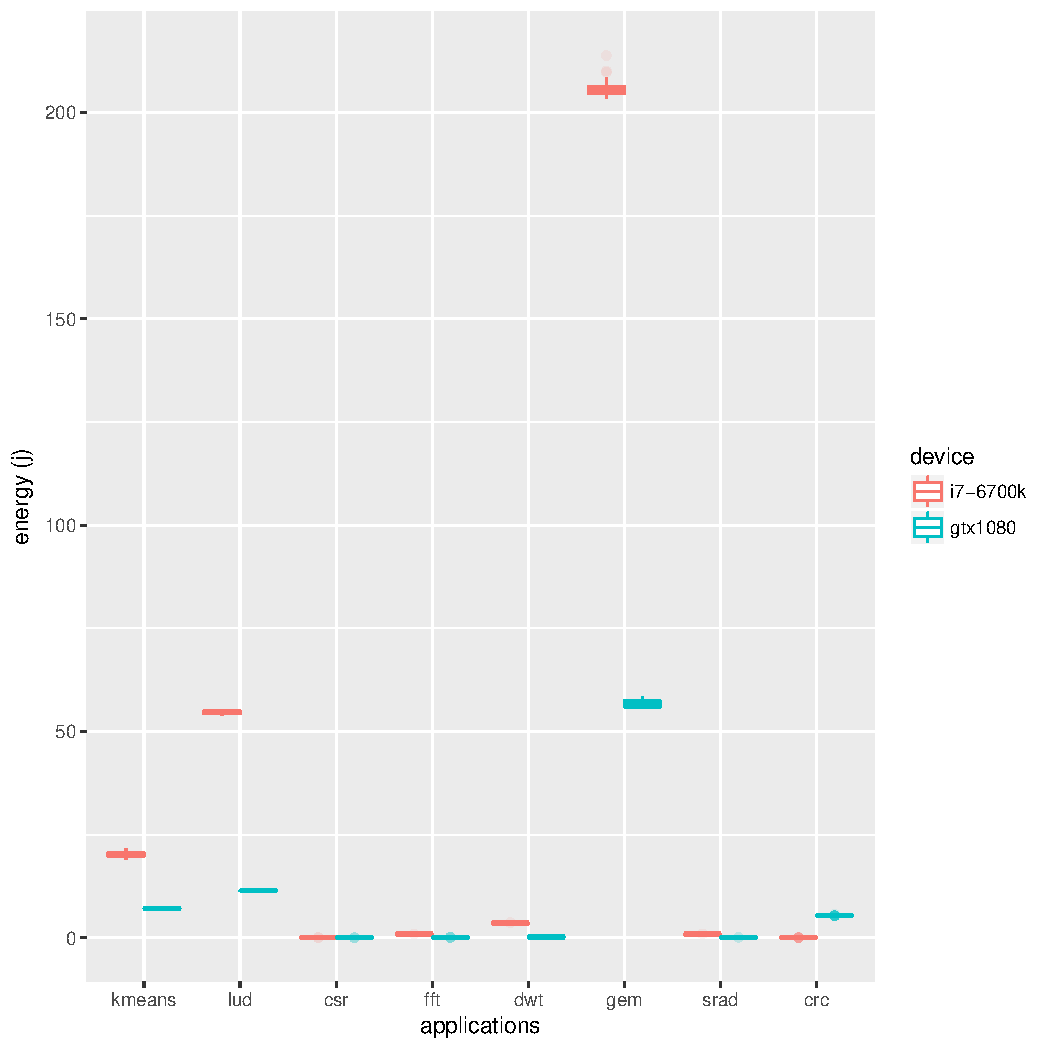
\includegraphics[width=1\textwidth]{figures/energy-results/energy_charts.pdf}
\caption{Kernel Execution energy}
\label{fig:energy}
\end{subfigure}
\hfill
\begin{subfigure}[htb]{.45\textwidth}
\centering
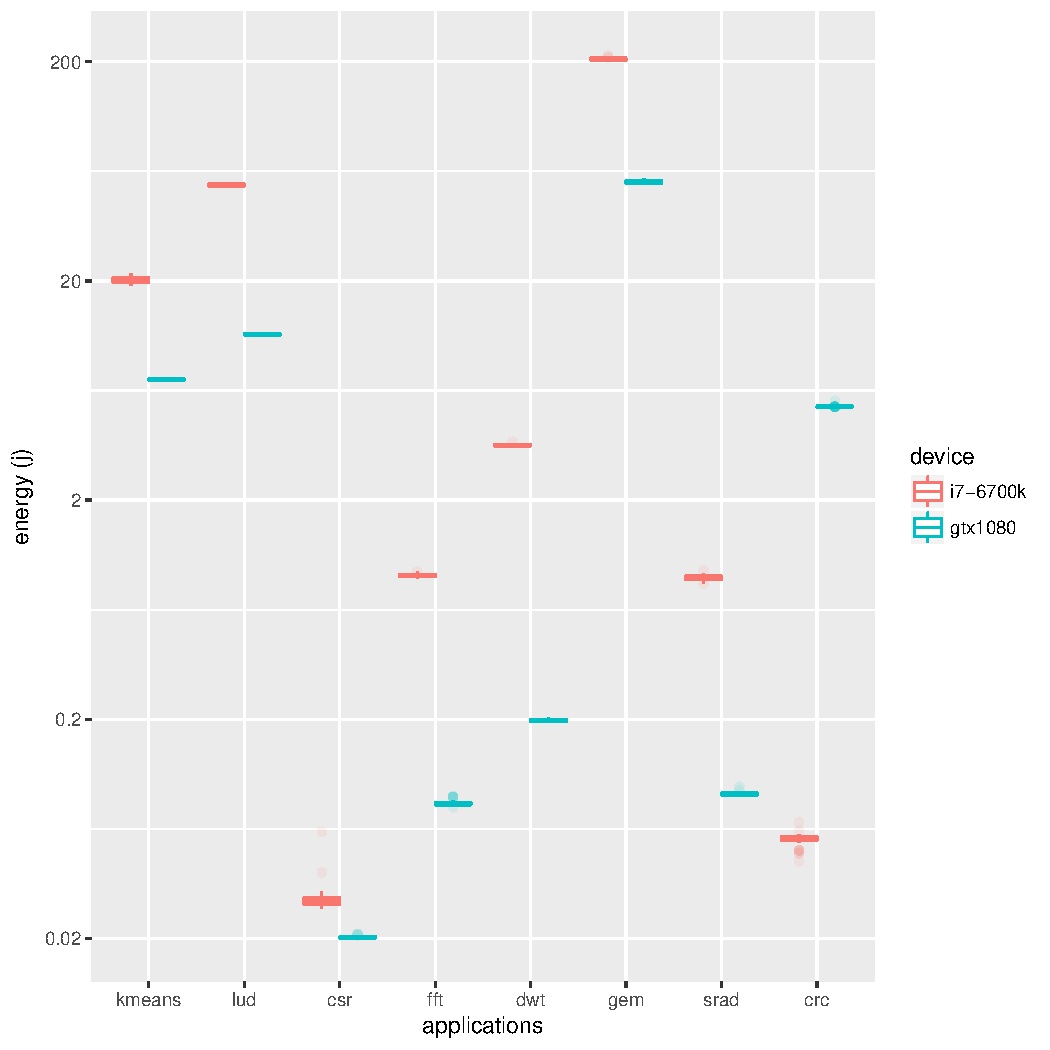
\includegraphics[width=1\textwidth]{figures/energy-results/energy_charts_log10.pdf}
\caption{Logarithmic Kernel Execution energy}
\label{fig:energy-log}
\end{subfigure}
\caption{Joules required to perform the kernel execution of all benchmark applications.}
\end{figure*}

\todo{Does energy scale with problem size for all benchmarks? Maybe not since dwarfs with large memory access cache misses could add huge overheads}

From the time results presented in Section~\ref{ssec:time} we see the largest difference occurs between CPU and GPU type accelerators at the {\bf large} problem size.
Thus we expect that the {\bf large} problem size will also show the largest difference in energy.
This is explored in Figures~\ref{fig:energy} and~\ref{fig:energy-log} where several applications are compared over the {\bf large} size.
All results are presented in joules.
Each pair of box plots has been grouped by colour according to device, red for the Intel Skylake i7-6700k CPU and blue for the Nvidia GTX1080 GPU.
These were the only devices examined since collection of RAPL and NVML PAPI performance measurements (with LibSciBench) requires super user access, and both these devices were the only accelerators available with this permission.
Nonetheless, certain trends become apparent when directly comparing joules required over a range of problems.
The logarithmic transformation has been applied to Figure~\ref{fig:energy-log} to emphasise the variation at the smaller energy scales (< \SI{1}{\joule}), this will be remedied in the future by avoiding the small execution times to perform some of the applications, in particular all algorithms will be rebalanced with respect to the {\bf gem} benchmark -- which has the longest running time -- to other {\bf large} application sizes by adding an additional compute loop which will add redundancy but will standardize the magnitude of results.

The distributions were collected by measuring solely the kernel execution over a distribution of 50 runs.
Variance with respect to energy usage is larger on the CPU, which is consistent to the execution time results.
When comparing 

\end{document}
